\newcommand{\CBh}[2]{\ensuremath{\partial_{#1} {#2}}}
\newcommand{\DBh}[2]{\ensuremath{\Delta_{#1} {#2}}}
\newcommand{\DTwo}[2]{\ensuremath{D_{2}\left( #1, #2 \right)}}
\newcommand{\DInf}[2]{\ensuremath{D_{\infty}\left( #1, #2 \right)}}
\newcommand{\TR}[1]{\ensuremath{{#1}^{\mkern-1.5mu\mathsf{T}}}}

\noindent\textbf{Introduction, useful notations and properties.}
The visibility normal estimator can be defined for different sizes $k$
of stars. Therefore, for such a given size $k$, we denote by
$\vec{n}^k_V(p)$ the \emph{$k$-visibility normal at point $p$}.
The objective of this section is to demonstrate under which conditions
the $k$-visibility normal estimation is a multigrid convergent normal
estimator.

We restrict our study to the digitizations of compact subsets $X$ of
$\R^d$, whose topological boundary $\partial X$ has positive reach
greater than $\rho > 0$. Let $h > 0$ be the digitization grid step
and let $X_h := X \cap \Z^d$ be the Gauss digitization of $X$ with
step $h$. Seeing the set $X_h$ as the union of hypercubes with edge
length $h$ and centered on points of $X_h$, we call its topological
boundary the {\em digitized boundary} $\CBh{h}{X}$ of $X$ of step
$h$. The intersection of $\CBh{h}{X}$ with $(h(\Z+\frac{1}{2}))^d$ is
denoted by $\DBh{h}{X}$ and its elements are called the {\em digital
pointels} of $\CBh{h}{X}$. They correspond to the digital sets $Z$
of the previous sections, and we study the visibility between pointels
of $\DBh{h}{X}$ within its $k$-Star.


Finally let $\xi$ be the orthogonal projector of $\R^d$ onto $\partial
X$, which is well defined for any point within the reach of $\partial
X$. In fact we only require points to be locally within the reach of
$\partial X$, so staying at distance below the \emph{local feature
size} (see \cite{amenta:2001-cgta}) is enough, but would require more
care in the theorem formulation and proofs. The following lemma will be useful.

\begin{lemma}{\cite{Lachaud:2016-jmiv}}
    \label{lem-hausdorff-close}
    Let $h$ be smaller than $\frac{2\rho}{\sqrt{d}}$.
    Let $p \in \CBh{h}{X}$. Then the point $p' := \xi(p)$ is at
    Euclidean distance from $p$ lesser or equal to
    $\frac{\sqrt{d}}{2}h$. Moreover $p'$ is the point of $\partial X$
    that is closest to $p$, and $(pp')$ is aligned with the normal of
    $\partial X$ at $p'$.
\end{lemma}

\noindent\textbf{Geometric properties on digitized boundary.}
The following theorem shows that the vector joining distant enough
points of the digitized boundary tend to be orthogonal to the smooth
boundary of $X$.
\begin{theorem}\label{bound-pq-dot-n}
    Let $h$ the gridstep be a positive number smaller than $h_0 :=
    \frac{2\rho}{\sqrt{d}}$. Let $p, q$ be two pointels of
    $\DBh{h}{X}$. It holds that:
    \begin{align}
        \label{eq-pq-dot-n-upper-bound}
        |\vec{pq} \cdot \vn| \Le \sqrt{d}h + \frac{(1+\sqrt{d})^2}{2}
        \frac{\|\vec{pq}\|^2}{\rho} + O\left(
                                           \frac{\|\vec{pq}\|^4}{\rho^3} \right),
    \end{align}
    where $\vn$ is the normal of $\partial X$ at $\xi(q)$.
\end{theorem}
\begin{proof}
    Since $h \le h_0$, both $p$ and $q$ are within the reach of
    $\partial X$ and have unique projection onto it. Let $p'=\xi(p)$,
    $q'=\xi(q)$. We consider the plane $P$ tangent to $\partial X$ at
    $q'$, with normal $\vec{n}$. Finally we denote by $p''$ the
    projection of $p'$ onto $P$. We have
    \begin{align*}
        | \vec{pq} \cdot \vn | & = | \vec{pp'} \cdot \vn  +  \vec{p'p''} \cdot \vn  + \vec{p''q'} \cdot \vn  +  \vec{q'q} \cdot \vn | \\
        & \quad \text{(By linearity of scalar product)}\\
        & \Le | \vec{pp'} \cdot \vn | + | \vec{p'p''} \cdot \vn | + |\vec{p''q'} \cdot \vn | + | \vec{q'q} \cdot \vn | \\
        & \quad \text{(by triangular inequality)} \\
        & \Le \| \vec{pp'} \| + \| \vec{p'p''} \| + 0 + \| \vec{q'q} \| \\
        & \quad \text{(since $\vec{p''q'}$ is parallel to $P$)}\\
        & \Le \sqrt{d}h + \| \vec{p'p''} \|. \\
        & \quad \text{(using \RefLemma{lem-hausdorff-close} twice)}
    \end{align*}

    Since $\partial X$ has positive reach greater than $\rho$, we know
    that $\partial X$ is sandwiched between two balls tangent to $P$ at
    $q'$. Their centers are $q' \pm \rho \vec{n}$. Let $c$ be the center
    of the ball that is on the same side of $P$ as $p'$, and let us
    denote $r$ the projection of $p'$ onto the line going through both
    ball centers (and $q$ and $q'$). From the sandwich property, $p'$
    cannot lie in any of these balls so $\| \vec{p'c} \| \Ge
    \rho$. Besides it holds that
    \begin{align*}
        \| \vec{p'c} \|^2 & = \| \vec{{p'}r} \|^2 + \| \vec{rc} \|^2 \\
        & \quad \text{(By Pythagoras theorem)} \\
        & = \| \vec{p''q'} \|^2 + \| \vec{rq'} +\vec{q'c} \|^2 \\
        & \quad \text{(by construction of $p''$ and $r$)} \\
        & = \| \vec{p''q'} \|^2 + ( \rho - \|\vec{p'p''}\|)^2. \\
        & \quad \text{(since $\vec{rq'}$ and $\vec{q'c}$ are aligned and $\vec{p'p''}=\vec{rq'}$)}
    \end{align*}
    With the lower bound $\| \vec{p'c} \| \Ge \rho$, it entails (with Taylor expansion):
    \begin{align*}
        \|\vec{p'p''}\| & \Le \rho - \sqrt{\rho^2 - \|\vec{p''q'} \|^2} \\
        & = \frac{1}{2}\frac{\|\vec{p''q'} \|^2}{\rho} + O \left( \frac{\|\vec{p''q'} \|^4}{\rho^3} \right).
    \end{align*}
    Now $\|\vec{p''q'} \| \Le \| \vec{p'q'} \| = \| \vec{p'p} + \vec{pq}
    + \vec{qq'} \| \Le \sqrt{d}h+\|\vec{pq}\| \Le
    (1+\sqrt{d})\|\vec{pq}\|$, the last inequality coming from the fact
    that $p \neq q$, so $1 \Le \frac{\|\vec{pq}\|}{h}$. We obtain:
    \begin{align*}
        \|\vec{p'p''}\| \Le \frac{(1+\sqrt{d})^2}{2}\frac{\|\vec{pq} \|^2}{\rho} + O \left( \frac{\|\vec{pq} \|^4}{\rho^3} \right).
    \end{align*}
    We conclude since we established above $| \vec{pq} \cdot \vn | \Le
    \sqrt{d}h + \| \vec{p'p''} \|$.
\end{proof}

\begin{figure}
    \centering
    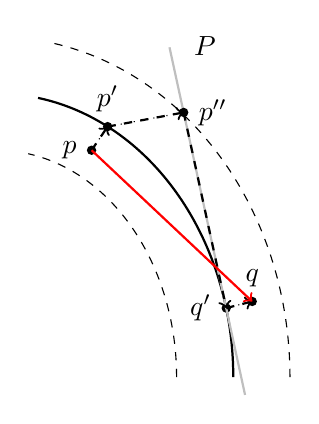
\begin{tikzpicture}[scale=1.2]

        \tikzset{
            surface/.style={thick},
            offset/.style={dashed},
            tangent/.style={thick, gray!50},
            proj/.style={dotted},
            vec/.style={->, thick,red},
            vecD/.style={->, thick, dashed},
            point/.style={circle, fill, inner sep=1.2pt}
        }

        \draw[surface]
        plot[domain=0:80,samples=100]
        ({2.5*cos(\x)}, {3*sin(\x)});

        \draw[offset]
        plot[domain=0:80,samples=100]
        ({2.5*cos(\x) + 0.6*cos(\x)},
            {3*sin(\x) + 0.6*sin(\x)});

        \draw[offset]
        plot[domain=0:80,samples=100]
        ({2.5*cos(\x) - 0.6*cos(\x)},
            {3*sin(\x) - 0.6*sin(\x)});


        \coordinate (p) at (1,2.4);
        \coordinate (q) at (2.7,0.8);

        \node[point,label=west:$p$] at (p) {};
        \node[point,label=above:$q$] at (q) {};

        \coordinate (pp) at (1.17,2.65);
        \coordinate (qq) at (2.425,0.73);

        \node[point,label=above:$p'$] at (pp) {};
        \node[point,label=left:$q'$] at (qq) {};

        \draw[proj] (p) -- (pp);
        \draw[proj] (q) -- (qq);

        \draw[tangent]
        plot[domain=-0.6:0.2]
        ({2.425+\x},{0.73-4.6*\x)});

        \node at (2.2,3.5) {$P$};

        \coordinate (ppp) at ({2.425+-0.45},{0.73-4.6*-0.45)});
        \node[point,label=right:$p''$] at (ppp) {};

        \draw[proj] (pp) -- (ppp);

        \draw[vecD] (p) -- (pp);
        \draw[vecD] (pp) -- (ppp);
        \draw[vecD] (ppp) -- (qq);
        \draw[vecD] (qq) -- (q);
        \draw[vec] (p) -- (q);

    \end{tikzpicture}
    \caption{Illustration of the 1st part of the proof of \RefTheorem{bound-pq-dot-n}.}
    \label{fig:fig-pq-dot-n-upper-bound}
\end{figure}

In order that the line $(pq)$ be at most orthogonal to the normal of
the smooth boundary, points $p$ and $q$ should not be too close
(otherwise there is a strong uncertainty on their positions) nor too
far away (the normal vector may vary too much). This is explicited in
the following corollary, which is immediate by dividing
\Equ{eq-pq-dot-n-upper-bound} by $\|\vec{pq}\|$.
\begin{corollary}
    \label{cor1}
    For $p \neq q$, let $\alpha$ be the angle between $\vec{pq}$ and $\vec{n}$. Then we have:
    \begin{align*}
        |\cos \alpha|
        % = \frac{|\vec{pq} \cdot \vn|}{\|\vec{pq}\|}
        \Le  \sqrt{d} \frac{h}{\|\vec{pq}\|} + \frac{(1+\sqrt{d})^2}{2}
        \frac{\|\vec{pq}\|}{\rho} + O\left(
                                         \frac{\|\vec{pq}\|}{\rho} \right)^3 \!\!.
    \end{align*}
    To minimize this value, it is optimal to choose pairs of points $(p,q)$ such that $\|\vec{pq}\|=\Theta(\sqrt{h})$. In this case, we derive $|\cos \alpha| \Le \Theta(\sqrt{h}) + O(\sqrt{h})^3$.
\end{corollary}

\noindent\textbf{Distance between visible points.}  This subsection
proves that the average distance between $k$-visible pointels is some
$\Theta(\sqrt{h})$, starting from $k\Ge 2$ for dimension 2 and 3.

\begin{lemma}\label{lem-segment-is-close-to-dX}
    Let $a,b$ be points of $\partial X$, where the straight line segment
    $\lbrack ab \rbrack$ has length $l$. If $l \Le 2\rho$ then $\max_{y
    \in \lbrack ab \rbrack} d(y, \partial X) \Le \frac{l^2}{4\rho}$,
    where $d(y,Z):=\inf_{z \in Z} \| y-z\|$.
\end{lemma}
\begin{proof}
    We recall that, since $\partial X$ has positive reach greater than
    $\rho$, it means that around point $a$, $\partial X$ has an empty
    intersection with the open ball of radius $\rho$ tangent to $a$
    (inside and outside). Therefore the distance $\max_{y \in \lbrack ab
    \rbrack} d(y, \partial X)$ cannot exceed the distance of a chord
    of length $l=\| \vec{ab}\|$ to a sphere of radius $\rho$, hence the
    circle of radius $\rho$ in the plane containing $a$, $b$ and the
    sphere center. By an abuse of notation, denoting $a$ and $b$ also
    the extremeties of this chord, $m$ its middle point, $c$ the center
    of the circle, and $p$ the closest point to $m$ on the circle, our
    objective is to determine the distance $x:=\| \vec{mp}\|$. Using the
    fact that $(cm)$ is orthogonal to $(ab)$, Pythagoras theorem implies
    $\|\vec{am}\|^2 + \|\vec{mc}\|^2 = \|\vec{ac}\|^2$. Substituting by
    $x$, $l$ and $\rho$ gives
    \begin{align*}
        \frac{l^2}{4}+(\rho-x)^2 = \rho^2 &
        \quad \Rightarrow \quad 4x^2 - 8 \rho x + l^2 = 0.
    \end{align*}
    Since $l \Le 2\rho$ by hypothesis, the solution to this equation is
    $x=\rho-\sqrt{\rho^2-\frac{l^2}{4}}$. To conclude, one can check
    easily that $x \Le \frac{l^2}{4\rho}$ if $l \Le
    2\rho$.
\end{proof}

\begin{theorem}\label{thm-distance-pq-to-dX}
    Let $p,q$ be two pointels of $\DBh{h}{X}$. If $\| \vec{pq}\|\Le
    \sqrt{\alpha h} - \sqrt{d}h$, then the segment $\lbrack p q \rbrack$
    stays close to $\CBh{h}{X}$ and more precisely:
    \begin{align*}
        \max_{r \in \lbrack p, q \rbrack} d( r, \CBh{h}{X}) \Le (\sqrt{d}+\frac{\alpha}{4\rho})h.
    \end{align*}
\end{theorem}
\begin{proof}
    Let $a=\xi(p)$ and $b=\xi(p)$ the (unique) projections of $a$ and
    $b$ onto $\partial X$. Then, by triangular inequality,
    \begin{align*}
        \max_{r \in \lbrack p q \rbrack} d( r, \CBh{h}{X})
        \Le & \max_{r \in \lbrack p q \rbrack} d( r, \lbrack a b \rbrack )
        + \max_{s \in \lbrack a b \rbrack} d( s, \partial X ) \\
        & + \max_{x \in \partial X} d( x, \CBh{h}{X} ).
    \end{align*}
    For the first term, we can write $r=(1-\lambda)p+\lambda q$, for
    some $\lambda \in \lbrack 0,1 \rbrack$. Let $s=(1-\lambda)a+\lambda
    b$. It is clearly a point of segment $\lbrack a b \rbrack$. We have:
    \begin{align*}
        d(r,s) & = \| (1-\lambda)p+\lambda q - ((1-\lambda)a+\lambda b) \| \\
        & \Le (1-\lambda)\|p-a\| + \lambda \|q-b\| \Le \frac{\sqrt{d}}{2}h,
    \end{align*}
    where the last inequality derives from
    \RefLemma{lem-hausdorff-close}.

    For the second term,
    \RefLemma{lem-segment-is-close-to-dX} induces
    \begin{align*}
        \max_{s \in \lbrack a b \rbrack} d( s, \partial X ) &\Le \frac{\|\vec{ab}\|^2}{4\rho}.
    \end{align*}
    But $\|\vec{ab}\| \Le \|\vec{ap}\| + \|\vec{pq}\| + \|\vec{qb}\| \Le
    \| \vec{pq}\| + \sqrt{d}h \Le \sqrt{\alpha h}$, using
    \RefLemma{lem-hausdorff-close} and the hypothesis on the distance of
    $p$ to $q$. The second term is thus bounded by $\frac{\alpha
    h}{4\rho}$.

    The last term is bounded by $\frac{\sqrt{d}}{2}h$
    (\RefLemma{lem-hausdorff-close} again), and the conclusion follows.
\end{proof}

\begin{theorem}
    \label{thm-k-visibility-distance}
    Assume $\alpha:=4\rho(k-\sqrt{d})$ is positive. Then, for any
    gridstep $h$, $0< h < \min(\frac{\alpha}{d}, 2\rho)$, there exists a
    constant $\beta >0 $ such that any two pointels of $\DBh{h}{X}$ at
    distance less than $\min(\beta \sqrt{h},2\rho)$ are $k$-visible.
    Furthermore the average distance between $k$-visible pointels of
    $\DBh{h}{X}$ is greater than $\Omega(\sqrt{h})$ for small enough
    $h$.
\end{theorem}
\begin{proof}
    Two pointels $p$ and $q$ are $k$-visible in $\DBh{h}{X}$ iff the
    segment $\lbrack p q \rbrack$ lies within the $k$-star of
    $\DBh{h}{X}$. Recalling that the realization in $\R^d$ of
    $\kStar{\DBh{h}{X}}{k}$ is exactly $\CBh{h}{X} \oplus k\rbrack -h, h
    \lbrack^d$ ($\oplus$ is the Minkowski sum), a sufficient condition
    is that
    \begin{align*}
        \max_{r \in \lbrack p q \rbrack} d(r,\DBh{h}{X}) \Le kh.
    \end{align*}
    Now let us fix $\beta:=\sqrt{\alpha}-\sqrt{dh}$. From $h <
    \frac{\alpha}{d}$, we have $\beta > 0$. If $\|\vec{pq}\| \Le \beta
    \sqrt{h}$, then $\|\vec{pq}\| \Le \alpha \sqrt{h} - \sqrt{d}h$.
    \RefTheorem{thm-distance-pq-to-dX} then implies
    \begin{align*}
        \max_{r \in \lbrack p, q \rbrack} d( r, \CBh{h}{X}) & \Le (\sqrt{d}+\frac{\alpha}{\
            4\rho})h \\
        & \Le \frac{4\rho\sqrt{d}+4\rho(k-\sqrt{d})}{4\rho}h\\
        & = kh,
    \end{align*}
    so $q$ is $k$-visible from $p$ in $\DBh{h}{X}$.

    We study now the average distance between $k$-visible pointels (in
    $\DBh{h}{X}$). Let $p$ be any pointel of $\DBh{h}{X}$. Let $V(p)$
    by the $k$-visible pointels from $p$, whose cardinal
    is denoted by $N(p)$. We subdivide $V(p)$ into three disjoint sets:
    $V_1(p)$ contains the $k$-visible pointels at distance less than
    $\beta \sqrt{h}/2$ (a non-empty set), $V_2(p)$ the ones at distance between $\beta
    \sqrt{h}/2$  and $\beta \sqrt{h}$ (a non-empty
    set), and $V_3(p)$ the remaining ones (which can be empty). Their
    respective cardinals are denoted by $N_i(p)$, $i\in \{1,2,3\}$.

    The average distance $D(p)$ of $k$-visible points from $p$ can be computed as:
    \begin{align*}
        D(p) & = \frac{1}{N(p)} \sum_{q \in V(p)} \|\vec{pq}\| \\
        & =\frac{1}{N(p)}  \left( \sum_{q \in V_1(p)} \hspace{-2mm}\|\vec{pq}\|
                               + \hspace{-2mm} \sum_{q \in V_2(p)} \hspace{-2mm}\|\vec{pq}\| + \hspace{-2mm} \sum_{q \in V_3(p)} \hspace{-2mm} \|\vec{pq}\|
        \right)\\
        & \Ge \frac{1}{N(p)} \left( N_2(p) \frac{\beta\sqrt{h}}{2} + N_3(p) \beta\sqrt{h} \right),
    \end{align*}
    by lower bounding the first term by $0$ and the third term by the
    minimal distance $\beta\sqrt{h}$. Now, since $\partial X$ is smooth
    and looks locally like a plane, the number of pointels of
    $\DBh{h}{X}$ in a ball centered at $p$ with radius $R$ is
    proportional to $R^{d-1} / h^{d-1}$. It coincides with the number of
    $k$-visible pointels from $p$ for $R = \beta \sqrt{h}$, since all
    these pointels are $k$-visible from $p$. It follows that
    $N_1(p)+N_2(p) \approx c N_2(p)$, with $c=\frac{2^{d}}{2^d-2}$ ($2$ in
    $2$D, $4/3$ in $3$D). Inserting into the previous inequality gives:
    \begin{align*}
        D(p) & \Ge \frac{1}{c
        N_2(p)+N_3(p)} \left(\frac{N_2(p)}{2}+N_3(p) \right) \beta\sqrt{h}\\
        & \Ge \frac{\beta}{2c}\sqrt{h}.
    \end{align*}
    We can conclude that the average distance $D(p)$ of $k$-visible
    points from $p$ is greater than $\Omega(\sqrt{h})$, since the last
    bound is valid for $c \Ge 1/2$, which is clearly the case for
    arbitrary dimension $d$.
\end{proof}

\textbf{Convergence of visibility normals.}  Let $V$ be a subset of
points of $\DBh{h}{X}$, whose distances to point $p \in \DBh{h}{X}$ lie in the
interval $\lbrack K_1 \sqrt{h}, K_2 \sqrt{h} \rbrack$, for $0< K_1
<K_2$ arbitrary constants, and $N$ be the cardinal of $V$. We define
the \emph{$V$-tangent matrix at $p$} as the symmetric positive definite
matrix
\begin{align*}
    A(p) & := \frac{1}{N}\sum_{q \in V} \frac{\vec{pq}}{\| \vec{pq} \|}
    \otimes \frac{\vec{pq}}{\| \vec{pq} \|}.
\end{align*}
The \emph{$V$-normal $\vec{n}_V(p)$ at $p$} is the last eigenvector of $A(p)$
(corresponding to the smallest eigenvalue). Note that we have not
required yet for $V$ to contain only points that are visible from $p$.

\begin{lemma}
    \label{lem-nAn-le-h}
    Let $\vn$ be the normal of $\partial X$ at $\xi(p)$.
    %% Assume $\alpha:=4\rho(k-\sqrt{d})$ is positive.
    Then, for any gridstep $h$
    smaller than $\frac{2\rho}{\sqrt{d}}$, the tensor $A(p)$ follows
    \begin{align*}
        0 \Le \TR{\vn} A(p) \vn \Le O(h).
    \end{align*}
\end{lemma}
\begin{proof}
    We develop $\TR{\vn} A(p) \vn$ as:
    \begin{align*}
        \TR{\vn} A(p) \vn & = \TR{\vn} \left( \frac{1}{N}\sum_{q \in V} \frac{\vec{pq}}{\| \vec{pq} \|} \otimes \frac{\vec{pq}}{\| \vec{pq} \|} \right) \vn \\
        & = \frac{1}{N} \sum_{q \in V} \left( \vn \cdot \frac{ \vec{p q} }{\|\vec{p q}\|} \right)^2\\
        & \Le \frac{1}{N} \sum_{q \in V} \left(O(\sqrt{h})\right)^2 = O(h),
    \end{align*}
    where the last inequality is a direct consequence of Corollary~\ref{cor1} (with the hypotheses of \RefTheorem{thm-k-visibility-distance}).
    %% We subdivide the $k$-visible points from $p$ into two subsets:
    %% $V_1$ contains the $k$-visible pointels at distance between $K_1
    %% \sqrt{h}$ and $\beta \sqrt{h}$ (a non-empty set), $V_2$ the ones at
    %% distance between $\beta \sqrt{h}$ and $K_2 \sqrt{h}$. Their
    %% respective cardinals are denoted by $N_1$ and $N_2$, and $N=N_1+N_2
    %% > 0$ (see proof of \RefTheorem{thm-k-visibility-distance}). We bound
    %% the two terms using Corollary~\ref{cor1}:
    %% \begin{align*}
    %% \frac{1}{N}\sum_{q \in V_1} \left( \vn \cdot \frac{ \vec{p q} }{\|\vec{p q}\|\
    %% } \right)^2 & \Le \frac{N_1}{N}\left(O(\sqrt{h})\right)^2 \\
    %% \frac{1}{N}\sum_{q \in V_2} \left( \vn \cdot \frac{ \vec{p q} }{\|\vec{p q}\|\
    %% } \right)^2 & \Le \frac{N_2}{N}\left(O(\sqrt{h})\right)^2.
    %% \end{align*}
    %% Both terms are bounded by $O(h)$, which proves the upper bound. The
    %% lower bound is true since $A(p)$ is SPD.
\end{proof}


\begin{theorem}
    \label{thm-angle-convergence}
    Assume $\alpha:=4\rho(k-\sqrt{d})$ is positive. Let $h$ be a
    gridstep smaller than $\min(\frac{\alpha}{d}, 2\rho)$. Let
    $\beta:=\sqrt{\alpha}-\sqrt{dh}$. Let $p$ be a digital point of
    $\DBh{h}{X}$. Let $V_k$ be the $k$-visible points from $p$ in
    $\DBh{h}{X}$, whose distance to $p$ lies in the interval $\lbrack
    K \sqrt{h}, \beta \sqrt{h} \rbrack$, with $K$ chosen such that
    $0< K< \beta$. Let $\vn$ be the normal of $\partial X$ at
    $\xi(p)$. Then the angle between $\vn$ and the last
    eigenvector $\vv_d$ of the $V_k$-tangent matrix $A(p)$ follows:
    \begin{align}
        \label{eq-alpha-upper-bound}
        \angle (\vv_d, \vn) \Le O\left(\sqrt{\frac{h}{\lambda_{d-1} - \lambda_d}}\right).
    \end{align}
    Furthermore $\lambda_{d-1} - \lambda_d >0$ and tends to $1/(d-1)$.
\end{theorem}
\begin{proof}
    Assuming the hypotheses, we have $\TR{\vn} A(p) \vn \Le \Theta(h)$
    according to \RefLemma{lem-nAn-le-h}. Now we can use
    \RefCorollary{cor2} (see \RefSection{sec-appendix},
    page~\pageref{sec-appendix}) with $\epsilon := \Theta(h)$ to obtain
    \Equ{eq-alpha-upper-bound} (the term in
    $O(\epsilon^{\frac{3}{2}})$).

    We must now study the eigenvalues of
    $A(p)$. According to \RefTheorem{thm-k-visibility-distance}, all the
    points of $\DBh{h}{X}$ at distance less or equal to $\beta \sqrt{h}$
    are visible from $p$. They form a regular sampling of a ring-like
    shape $R_h$ in-between the balls centered on $p$ and of radii
    $K\sqrt{h}$ and $\beta\sqrt{h}$, and the two planes orthogonal to
    $\vn$ around $p$, lying at a distance $O(h)$.

    Indeed, if $P$ is the tangent plane at $\xi(p)$ to $\partial X$ (hence
    orthogonal to $\vn$), \cite[Lemma~10]{Boissonnat:2019-jact} tells
    that $\forall a,b \in \partial X, d(b, P) \le
    \frac{\|a-b\|^2}{\rho}$. Let $a=\xi(p)$ and $b=\xi(q)$ for $q in
    V_k$. Since $\|a-p\|=O(h)$, $\|b-q\|=O(h)$, and
    $\|p-q\|=\Theta(\sqrt{h})$, we have first that
    $\|a-b\|=O(\sqrt{h})$. Then it holds that
    \begin{align*}
        d(q, P) \Le \|q-b\| + d(b,P) \Le O(h) + \frac{O(\sqrt{h})^2}{\rho}
        = O(h).
    \end{align*}
    So any $q \in V_k$ lies in-between two planes orthogonal to $\vn$
    around $p$, lying at a distance $O(h)$, hence in the ring $R_h$.

    In an orthonormal basis $(\vv_i)_{i=1,\ldots,d}$,
    whose last vector $\vv_d$ is equal to $\vn$, the coordinates of
    vector $\vec{pq_j}$, $q_j \in V_k$, follow $(O(\sqrt{h}), \ldots,
    O(\sqrt{h}), O(h))$. Hence, letting
    $\vu_i:=\frac{\vec{pq_j}}{\|\vec{pq_j}\|}$, their coordinates follow
    $(O(1), \ldots, O(1), O(\sqrt{h}))$. This shows that the last
    eigenvalue $\lambda_d$ of $A(p)$ tends to $0$ as $h$ tends to $0$.

    Finally all the unit vectors $\vu_i$ sample the directions of an
    isotropic ring-shape that is squeezed more and more into a 2d
    ring. It means that they sample more and more precisely the
    $d-1$-sphere of radius $1$ belonging to the plane orthogonal to
    $\vn$ centered on $\mathbf{0}$. The eigenvectors thus tend to an
    abritrary orthonormal basis of this plane, while the $d-1$ largest
    eigenvalues tend to the same value. As shown in
    \RefSection{sec-appendix}, the sum of all eigenvalues is 1, so every
    eigenvalue $\lambda_1, \ldots, \lambda_{d-1}$ tends to
    $\frac{1}{d-1}$.
\end{proof}

\begin{corollary}
    \label{cor-convergence}
    With the hypotheses of \RefTheorem{thm-angle-convergence}, the
    $V_k$-visibility normal is a multigrid convergent normal estimator,
    with convergence speed in $O(\sqrt{h})$.
\end{corollary}

\begin{remark}
    Since $\alpha$ must be positive, the $V_k$-visibility normal estimation is
    convergent for $k \ge 2$ in $2$d and $3$d. For higher dimensions up to $8$, the
    $V_k$-visibility normal estimation is convergent for $k \ge 3$.
\end{remark}
\begin{remark}
    In practice, we know only approximately the reach of the shape under
    study, so choosing constants $K$ and $\beta$ is not handy. Instead,
    we sort the $V_k$-visible points from $p$ according to their
    distance to $p$, and we simply keep the half of the points whose
    distance are closest to the average distance. Since we know that the
    average distance to $p$ is greater than some $\Omega(\sqrt{h})$
    (\RefTheorem{thm-k-visibility-distance}), keeping this half is a
    good approximation of the targeted hypotheses for
    convergence. Furthermore, it avoids the necessity of setting
    parameters.
\end{remark}
%% We slightly simplify here
%% the definition of the $k$-visibility normal $\vec{n}_k(p)$ at point
%% $p$ by removing the weights and by centering the tensor matrix at
%% point $p$. Let $V$ be the set of $k$-visible points in $\DBh{h}{X}$
%% from $p$, whose distances lie in the interval $\lbrack K_1 \sqrt{h},
%% K_2 \sqrt{h} \rbrack$. From a theoretical perspective, constants $K_1$
%% and $K_2$ should satisfy $0 < K_1 < \beta < K_2$. The value $\beta$ is
%% chosen according to \RefTheorem{thm-k-visibility-distance} as
%% $2\sqrt{k - \sqrt{d}}\sqrt{\rho} -\sqrt{dh}$. From a practical point
%% of view, we sort the $k$-visible points from $p$ according to their
%% distance to $p$, and we simply keep the half of the points whose
%% distance are closest to the median distance.


%% \begin{remark}
%%   Constants for $O$ notations are respectively:
%%   $\frac{\sqrt{d}}{K_1}+(1+\sqrt{d})^2\sqrt{\frac{k-\sqrt{d}}{\rho}}$
%%   and
%%   $\frac{\sqrt{d}}{2\sqrt{\rho(k-\sqrt{d})}}+\frac{K_2(1+\sqrt{d})^2}{2\rho}$.
%% \end{remark}
